\begin{frame}{Roadmap}

\begin{itemize}
\tightlist
\item
  RMINC history
\item
  CRAN
\item
  Software development and design
\item
  RMINC under the hood

  \begin{itemize}
  \tightlist
  \item
    representations
  \item
    abstractions
  \end{itemize}
\item
  Getting RMINC ready for CRAN

  \begin{itemize}
  \tightlist
  \item
    building
  \item
    testing
  \item
    documenting
  \item
    standardizing
  \end{itemize}
\item
  Future Directions
\end{itemize}

\end{frame}

\begin{frame}{RMINC}

\begin{itemize}
\tightlist
\item
  R interface to the world of MINC
\item
  Statistics for minc volumes
\item
  First commit in 2005!
\item
  Version 1.3 released February 25th, 2016
\end{itemize}

\end{frame}

\begin{frame}{Inception}

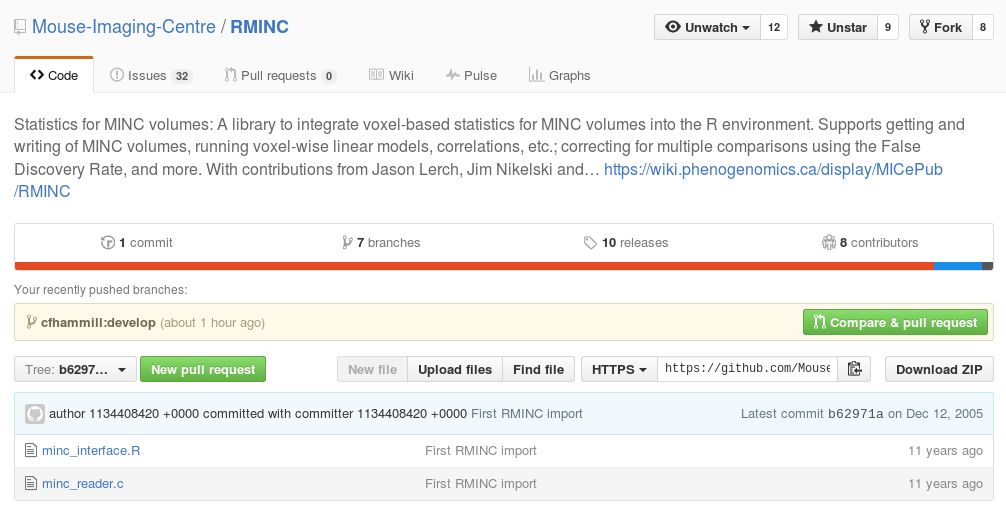
\includegraphics{RMINC_commit_one.png}

\end{frame}

\begin{frame}{Development}

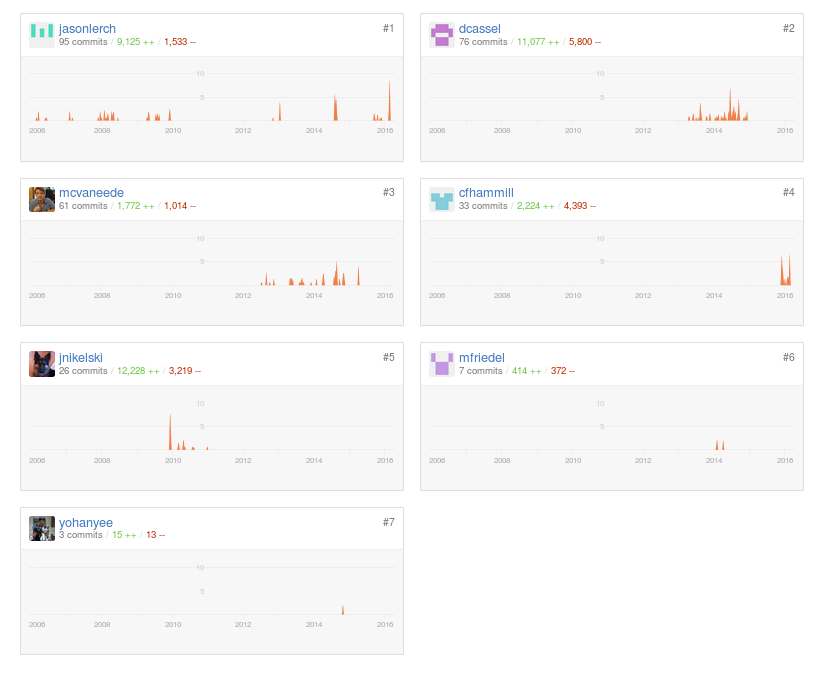
\includegraphics{contributors.png}

\end{frame}

\begin{frame}{Most Recent Release}

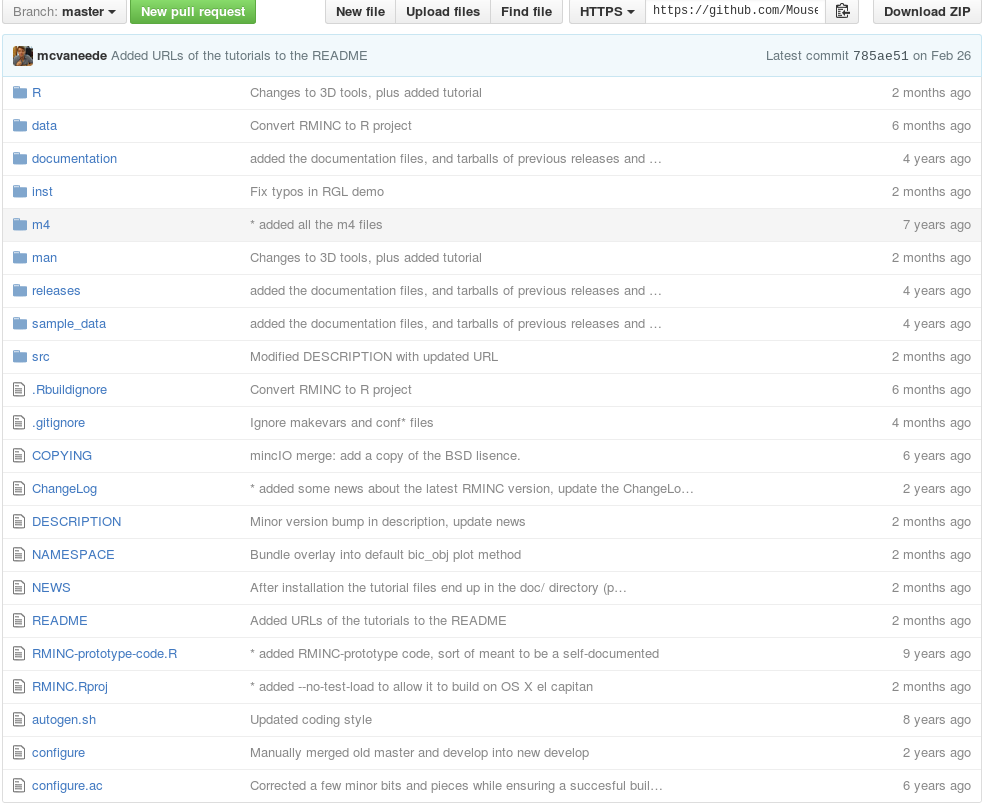
\includegraphics{RMINC_recent_master.png}

\end{frame}

\begin{frame}{Most Recent Development Branch}

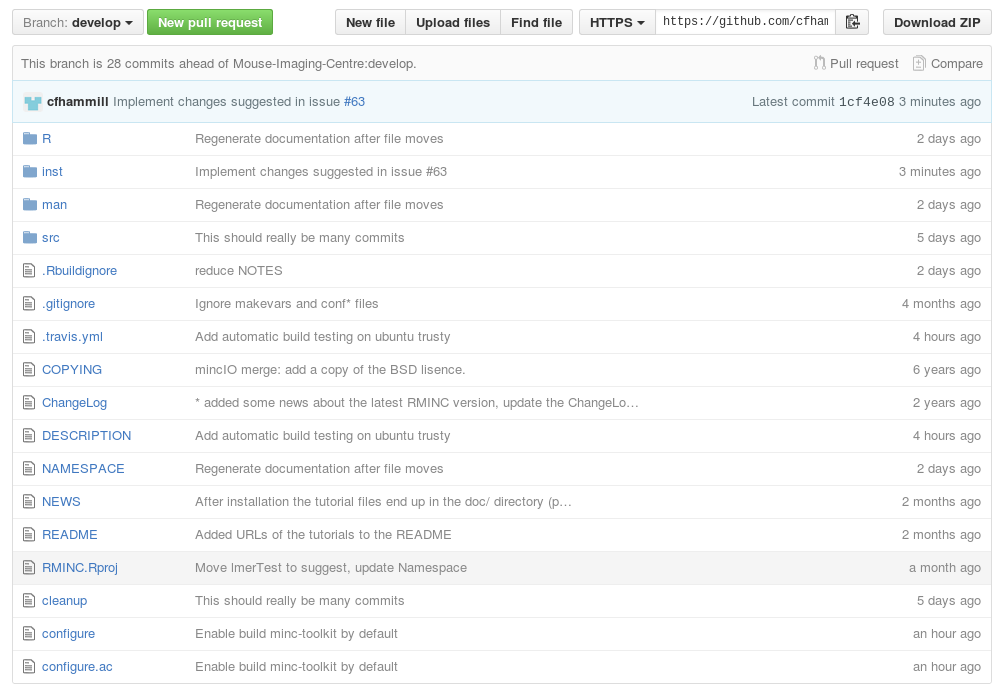
\includegraphics{RMINC_recent_dev.png}

\end{frame}

\begin{frame}{Improving accessibility}

\begin{itemize}[<+->]
\tightlist
\item
  Visibility (be on CRAN)
\item
  Availability (be on CRAN)
\item
  Ease of install (be on CRAN)
\item
  Working toward a CRAN release
\end{itemize}

\end{frame}

\begin{frame}{CRAN}

\begin{itemize}
\tightlist
\item
  The Comprehensive R Archive Network
\item
  8287 Packages
\item
  Holds all major R packages
\item
  Run by the R-project
\item
  Pretty high standards
\end{itemize}

\end{frame}

\begin{frame}{Package Development}

\begin{itemize}[<+->]
\tightlist
\item
  \textbf{Scripting vs.~Software Development}
\item
  getting the job done vs.~building a system
\item
  comes down to design
\end{itemize}

\end{frame}

\begin{frame}{Symptoms of design problems}

\begin{itemize}[<+->]
\tightlist
\item
  \textbf{Rigid}: \newline
     tedency for code to resist modification
\item
  \textbf{Fragile}: \newline
     tendency for modifications to break code in unexpected places
\item
  \textbf{Immobile}: \newline
     tendency for supposedly modular code to not work in new situations
\item
  \textbf{Viscous}: \newline
     tendency for hacks to be easier to implement than robust
  solutions\footnote<.->{Metaphors from Robert Martin}
\end{itemize}

\end{frame}

\begin{frame}{Design focuses}

\begin{itemize}
\tightlist
\item
  Design revolves around data
\item
  \textbf{Representation}
\item
  \textbf{Abstraction}
\end{itemize}

\end{frame}

\begin{frame}{Barriers to good design}

\begin{itemize}
\tightlist
\item
  Cruft
\item
  Maintaining compatibility
\item
  Complexity
\item
  Managing dependencies and interfacing with external code
\end{itemize}

\end{frame}

\begin{frame}{Refactoring}

\begin{itemize}
\tightlist
\item
  Work to make code more understandable
\item
  Work to make code easier to maintain
\item
  Focus on writing small reliable functions
\item
  Focus on composability
\item
  Minimize global state
\end{itemize}

\end{frame}

\begin{frame}{RMINC}

\begin{block}{Representations for minc files}

\end{block}

\begin{block}{Abstractions for performing statistics}

\end{block}

\end{frame}

\begin{frame}{Representations}

\begin{itemize}
\tightlist
\item
  \texttt{mincSingleDim}: flat vector of intensities for single minc
  files and single value statistics tagged with metadata
\item
  \texttt{mincMultiDim}: matrices with columns corresponding typically
  to different statistics, tagged with metadata
\item
  \texttt{mincArray}: 3D array of intensities for a single minc file
\item
  \texttt{mincMultiArray}?: Dimension respecting representations for
  results modelling
\end{itemize}

\end{frame}

\begin{frame}{Abstraction Goals}

\begin{itemize}
\tightlist
\item
  Facilitate movement of imaging data to and from the file system
\item
  Facilitate the generation of useful representations
\item
  Facilitate the fitting of statistical models
\item
  Reduce iteration time for data exploration
\end{itemize}

\end{frame}

\begin{frame}{Abstraction Goals}

\begin{itemize}
\tightlist
\item
  Facilitate movement of imaging data to and from the file system
\item
  Facilitate the generation of useful representations
\item
  \textbf{Facilitate the fitting of statistical models}
\item
  \textbf{Reduce iteration time for data exploration}
\end{itemize}

\end{frame}

\begin{frame}[fragile]{Easy Model Fitting}

\begin{itemize}[<+->]
\tightlist
\item
  Modelling in R is typically direct
\end{itemize}

\begin{Shaded}
\begin{Highlighting}[]
\KeywordTok{glm}\NormalTok{(binomial_response ~}\StringTok{ }\NormalTok{covariate1 +}\StringTok{ }\NormalTok{... +}\StringTok{ }\NormalTok{covariateN, }
    \DataTypeTok{data =} \NormalTok{data_source, }
    \DataTypeTok{family =} \NormalTok{binomial )}
\end{Highlighting}
\end{Shaded}

\begin{itemize}[<+->]
\tightlist
\item
  \textbf{Challenge}: a full experiment will not fit in memory
\item
  \textbf{Solution}: iterate through files extracting vectors of voxel
  values those voxel values are then fit against covariates
\end{itemize}

\end{frame}

\begin{frame}

\footnote<.->{Mouse icon made by Freepik from www.flaticon.com}

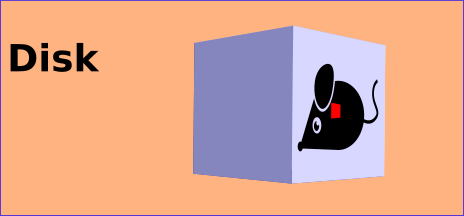
\includegraphics{minc_file_icon.png}

\end{frame}

\begin{frame}

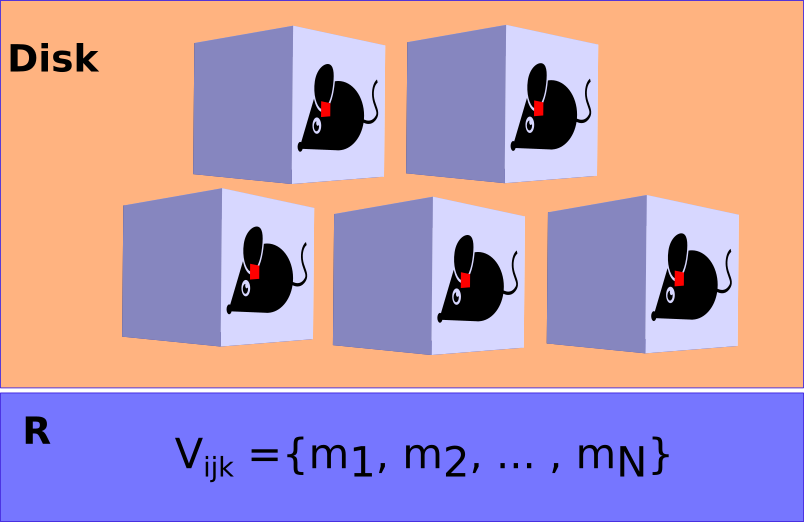
\includegraphics{mouse_vector1.png}

\end{frame}

\begin{frame}

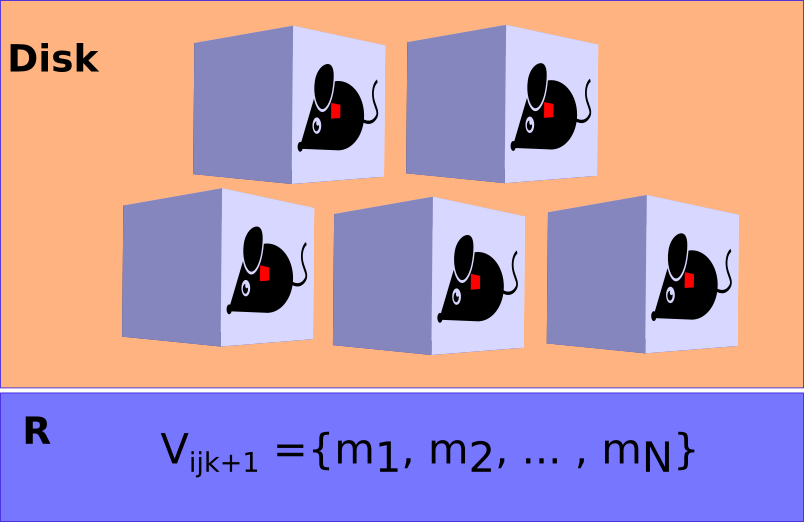
\includegraphics{mouse_vector2.png}

\end{frame}

\begin{frame}{Fitting models}

\begin{itemize}
\tightlist
\item
  Abstractions:

  \begin{itemize}
  \tightlist
  \item
    \texttt{mincLm}
  \item
    \texttt{mincLmer}
  \item
    \texttt{mincAnova}
  \item
    \texttt{mincTtest} \newline
    \ldots{}
  \item
    \texttt{mincApply}
  \item
    \texttt{mincApplyRCPP}
  \end{itemize}
\end{itemize}

\end{frame}

\begin{frame}[fragile]{mincApplyRCPP}

\begin{itemize}
\tightlist
\item
  R fluent interface to applying over voxels
\end{itemize}

\begin{Shaded}
\begin{Highlighting}[]
\KeywordTok{str}\NormalTok{(}\KeywordTok{args}\NormalTok{(mincApplyRCPP))}
\end{Highlighting}
\end{Shaded}

\begin{verbatim}
## function (filenames, fun, 
##     ..., mask = NULL, maskval = NULL, 
##     filter_masked = FALSE, 
##     slab_sizes = c(1, 1, 1), 
##     return_indices = FALSE, 
##     collate = simplify2minc)
\end{verbatim}

\begin{Shaded}
\begin{Highlighting}[]
\KeywordTok{mincApplyRCPP}\NormalTok{(experiment_frame$filenames, sample, }\DataTypeTok{size =} \DecValTok{5}\NormalTok{)}
\end{Highlighting}
\end{Shaded}

\end{frame}

\begin{frame}{Expedite fitting models}

\begin{itemize}
\tightlist
\item
  \textbf{Challenge}: R is (generally) slow, fitting models can be slow
\item
  \textbf{Solution}: Implement parallelism
\item
  Abstractions:

  \begin{itemize}
  \tightlist
  \item
    \texttt{pMincApply}: General purpose parallelism
  \item
    \texttt{mcMincApply}: Multicore parallelism
  \item
    \texttt{qMincApply}: Grid computing parallelism
  \item
    \texttt{gMincApply}: Open problem
  \end{itemize}
\end{itemize}

\end{frame}

\begin{frame}{Dealing with clusters}

\begin{itemize}
\tightlist
\item
  Implements flexible support for multiple parallelism backends
\item
  Integration with `BatchJobs' package
\item
  So far works with HPF and our local cluster, \emph{should} work on
  scinet but it hasn't been tested
\item
  New abstractions allow computation to performed in the background
\end{itemize}

\end{frame}

\begin{frame}{New Cluster Abstractions}

\begin{itemize}
\tightlist
\item
  \texttt{qMincApply}: Turnkey function
\item
  \texttt{qMincRegistry}: Create shared files for parallel jobs to be
  coordinated, once created, registries can be loaded from another R
  session or even another machine
\item
  \texttt{qMincMap}: Split the calculation into many peices and prepare
  the scripts necessary for job submission
\item
  \texttt{qMincReduce}: Retrieve the job results combining them into the
  object of your choice, defaults to minc statistic object like
  \texttt{mincMultiDim}
\item
  Currently only performs voxel-wise calculations, but can be extended
  to more complex analyses or be used to parellelize hyper-parameter
  search
\end{itemize}

\end{frame}

\begin{frame}{Push for CRAN}

\begin{itemize}
\tightlist
\item
  Must build automatically on two platforms
\item
  Must perform as expected
\item
  Must be well documented
\item
  Must adhere to CRAN standards
\end{itemize}

\end{frame}

\begin{frame}[fragile]{Building R Packages}

\begin{itemize}
\tightlist
\item
  R uses a C-like build system
\item
  Supports basic configure scripts and makevars
\item
  Does not support cmake
\item
  \textbf{Challenge}: Locating/Providing system dependencies
\item
  \textbf{Solution(?)}: Using autoconf to generate a configure script
  that can flexibly locate libminc and hdf5
\item
  if they are not found it can build minc-toolkit-v2 from source using
  git and cmake (fraught for automatic builds)
\item
  \textbf{Goal}:
\end{itemize}

\begin{Shaded}
\begin{Highlighting}[]
\KeywordTok{install.packages}\NormalTok{(}\StringTok{"RMINC"}\NormalTok{)}
\end{Highlighting}
\end{Shaded}

Should work without issue from all supported platforms

\end{frame}

\begin{frame}{Keeping things working}

\begin{itemize}
\tightlist
\item
  Ensuring code performs as expected is a significant problem
\item
  Strategies exist to ensure code performs as expected
\end{itemize}

\end{frame}

\begin{frame}{Scale of Testing}

\begin{quote}
Optimism is an occupational hazard of programming: feedback is the
treatment - Kent Beck
\end{quote}

\begin{enumerate}
\def\labelenumi{\arabic{enumi}.}
\tightlist
\item
  \textbf{Optimism} - ``this really looks like it should work''
\item
  \textbf{Hand testing} - ``I tried a few variants of this and they
  work''
\item
  \textbf{Unit testing} - ``I broke the problem into small pieces, and
  had the computer check that they all work''
\item
  \textbf{Property testing} - ``I specified rules about return values,
  the computer explores parameter space to see if rules hold''
\item
  \textbf{Formal proof} - ``I mathematically demonstrated the program is
  correct''
\end{enumerate}

\end{frame}

\begin{frame}{Scale of Testing}

\begin{quote}
Optimism is an occupational hazard of programming: feedback is the
treatment - Kent Beck
\end{quote}

\begin{enumerate}
\def\labelenumi{\arabic{enumi}.}
\tightlist
\item
  \textbf{Optimism} - ``this really looks like it should work''
\item
  \textbf{Hand testing} - ``I tried a few variants of this and they
  work''
\item
  \textbf{Unit testing - ``I broke the problem into small pieces, and
  had the computer check that they all work''}
\item
  \textbf{Property testing} - ``I specified rules about return values,
  and had the computer explores parameter space to see if rules hold''
\item
  \textbf{Formal proof} - ``I mathematically demonstrated the program is
  correct''
\end{enumerate}

\end{frame}

\begin{frame}[fragile]{Unit testing}

\begin{itemize}
\tightlist
\item
  Unit tests are a set of assertions about the value functions return.
\end{itemize}

\begin{Shaded}
\begin{Highlighting}[]
\KeywordTok{library}\NormalTok{(testthat)}
\KeywordTok{test_that}\NormalTok{(}\StringTok{"My Code Works"}\NormalTok{,}
           \KeywordTok{expect_equal}\NormalTok{(}\KeywordTok{mean}\NormalTok{(}\DecValTok{1}\NormalTok{:}\DecValTok{5}\NormalTok{), }\DecValTok{3}\NormalTok{))}

\KeywordTok{test_that}\NormalTok{(}\StringTok{"My other code also works"}\NormalTok{,}
         \KeywordTok{expect_equal}\NormalTok{(}\KeywordTok{sd}\NormalTok{(}\DecValTok{1}\NormalTok{:}\DecValTok{5}\NormalTok{), }\FloatTok{1.5}\NormalTok{))}
\end{Highlighting}
\end{Shaded}

\begin{verbatim}
## Error: Test failed: 'My other code also works'
## Not expected: sd(1:5) not equal to 1.5
## 1.58 - 1.5 == 0.0811.
\end{verbatim}

\end{frame}

\begin{frame}[fragile]{RMINC Testing}

\begin{itemize}
\tightlist
\item
  RMINC includes a tool for testing the package
\end{itemize}

\begin{Shaded}
\begin{Highlighting}[]
\KeywordTok{runRMINCTestbed}\NormalTok{()}
\end{Highlighting}
\end{Shaded}

runs a suite of tests on our code to check that all is working as
expected

\begin{itemize}
\tightlist
\item
  \texttt{runRMINCTestbed} calls out to `test\_directory' which runs all
  tests in \texttt{inst/tests}
\item
  Canonical approach is to have tests in \texttt{test} so that CRAN can
  test them automatically, but some thought is needed on how best to do
  the conversion
\end{itemize}

\end{frame}

\begin{frame}{Integration testing}


\includegraphics{travis_ci.png}

\begin{itemize}
\tightlist
\item
  Services provide automatic testing on multiple platforms
\item
  Runs whenever code is changed on github
\item
  Runs whenever a pull request is issued
\end{itemize}

\end{frame}

\begin{frame}{R Documentation}

\begin{itemize}[<+->]
\tightlist
\item
  CRAN requires all user visible functions to be documented. \newline
    This is huge benefit to users as all documentation can be quickly
  accessed with the standard \texttt{?} call
\item
  \textbf{Challenge}: Documentation must be kept in sync with the code
\item
  \textbf{Solution}: Documentation lives in source with the code and is
  autogenerated each time the package is rebuilt.\newline 
\item
  `roxygen2' integration with rstudio supports this
\end{itemize}

\end{frame}

\begin{frame}[fragile]{Roxygen Documentation}

\begin{Shaded}
\begin{Highlighting}[]
\CommentTok{#' Retrieve Voxel Values}
\CommentTok{#' }
\CommentTok{#' Return the intensity of a given voxel in a set of minc files}
\CommentTok{#' }
\CommentTok{#' @param filenames paths to the minc files}
\CommentTok{#' @param v1 Either a 3-element vector of voxel coordinates }
\CommentTok{#' or the first}
\CommentTok{#' @param v2 the second voxel coordinate if not NULL}
\CommentTok{#' @param v3 the third voxel coordinate if not NULL}
\CommentTok{#' @return Returns a \textbackslash{}code\{mincVoxel\} object containing a vector}
\CommentTok{#' of intensities and attributes specify the voxel and world }
\CommentTok{#' coordinates of the values.}
\CommentTok{#' @export}
\NormalTok{mincGetVoxel <-}\StringTok{ }\NormalTok{function(filenames, v1, }\DataTypeTok{v2=}\OtherTok{NULL}\NormalTok{, }\DataTypeTok{v3=}\OtherTok{NULL}\NormalTok{) \{}
\end{Highlighting}
\end{Shaded}

\end{frame}

\begin{frame}

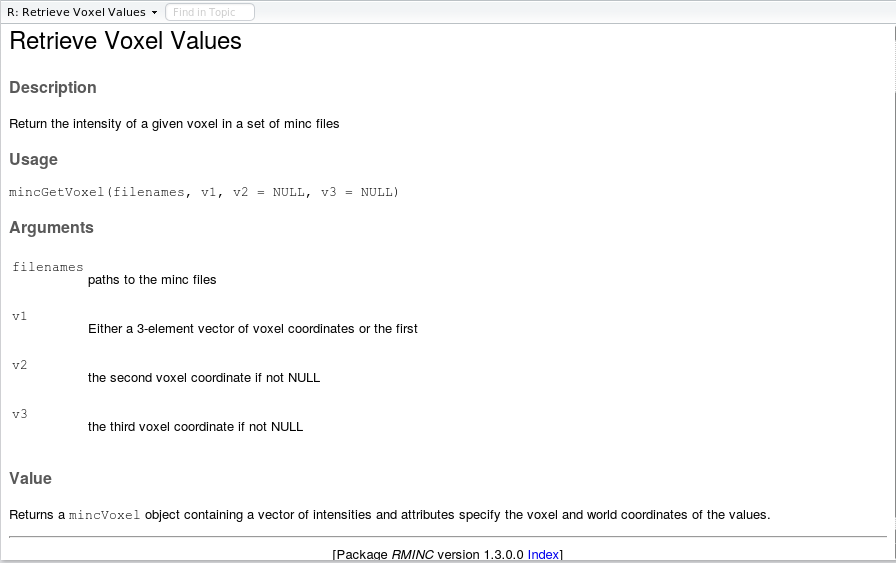
\includegraphics{mincGetVoxelRD.png}

\end{frame}

\begin{frame}{Appeasing R CMD check}

\begin{itemize}
\tightlist
\item
  CRAN is very particular about code quality
\item
  Luckily R CMD check tests many requirements for you
\item
  Highlights missed arguments in documentation, missing global variables
  (helpful for catching typos)
\item
  Ensures dependencies can be loaded properly
\end{itemize}

\end{frame}

\begin{frame}{Future directions}

\begin{itemize}
\tightlist
\item
  Almost ready for release
\item
  Harden parallel code
\item
  Convert testing scheme to canonical approach
\item
  Add abstractions for multivariate statistics
\end{itemize}

\end{frame}

\begin{frame}

\centering{\Large{Ever need R help? \newline Come by my desk or drop me an email}}

\end{frame}

\begin{frame}

\centering{\Large{Questions?}}

\end{frame}
